\chapter{Integrální počet}

\section{Definice integrálu}

Zaveďme pojem plocha pod křivkou. Mějme funkci \(y = \mathrm{f}(x)\) definované na intervalu \(<a, b>\). Plochou pod křivkou funkce \(\mathrm{f}(x)\) rozumíme plochu mezi křivkou určenou touto funkcí a~osou \(x\) omezenou na interval \(<a, b>\). Tato plocha je kladná pokud jsou hodnoty funkce kladné (křivka leží nad osou \(x\)) nebo záporná pokud jsou hodnoty funkce záporné (křivka leží pod osou \(x\)).
Na obrázku~\ref{img:plocha_pod_krivkou} je tato plocha zobrazena šedou barvou.

\begin{figure}[ht]
\begin{center}
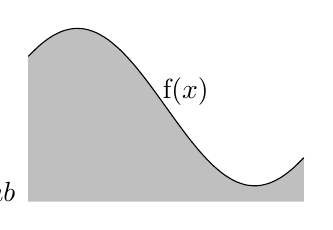
\begin{tikzpicture}
\path [smooth, domain=0.5:4, fill=lightgray]
 plot({\x}, {1.2 + sin(80 * \x)})
  -- (4, 0) -- (0.5, 0) -- (0.5, 1.2);
  
\draw [smooth, domain=0.5:4] plot({\x}, {1.2 + sin(80 * \x)});
\draw (2.5, 1.4) node{\(\mathrm{f}(x)\)};

\drawaxesxy{0}{0}{-0.5}{-0.5}{4.5}{2.5}

\drawxcoord{0.5}{0}{\(a\)}
\drawxcoord{4}{0}{\(b\)}

\end{tikzpicture}
\caption{Plocha pod křivkou}
\end{center}
\label{img:plocha_pod_krivkou}
\end{figure}

Označme tuto plochu pod křivkou

\begin{equation}
\int_{a}^{b} \mathrm{f}(x) \cdot \mathrm{d}x
\end{equation}

a~nazvěme ji určitý integrál.

Prozkoumejme, jaké vlastnosti má určitý integrál. Zaprvé se plocha pod křivkou pro sousední intervaly sčítá jak je vidět na obrázku~\ref{img:scitani_integralu}, tedy

\begin{equation}
\label{eq:scitani_integralu}
\int_{a}^{c} \mathrm{f}(x) \cdot \mathrm{d}x + \int_{c}^{b} \mathrm{f}(x) \cdot \mathrm{d}x = \int_{a}^{b} \mathrm{f}(x) \cdot \mathrm{d}x
\end{equation}

\begin{figure}[ht]
\begin{center}
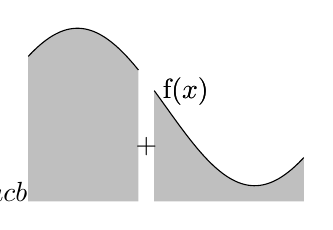
\begin{tikzpicture}
\path [smooth, domain=0.5:1.9, fill=lightgray]
 plot({\x}, {1.2 + sin(80 * \x)})
  -- (1.9, 0) -- (0.5, 0) -- (0.5, 1.2);
  
\draw [smooth, domain=0.5:1.9] plot({\x}, {1.2 + sin(80 * \x)});
\draw (2.5, 1.4) node{\(\mathrm{f}(x)\)};


\path [smooth, domain=2.1:4, fill=lightgray]
 plot({\x}, {1.2 + sin(80 * \x)})
  -- (4, 0) -- (2.1, 0) -- (2.1, 1.2);
  
\draw [smooth, domain=2.1:4] plot({\x}, {1.2 + sin(80 * \x)});
\draw (2.5, 1.4) node{\(\mathrm{f}(x)\)};

\draw (2, 0.7) node{+};

\drawaxesxy{0}{0}{-0.5}{-0.5}{4.5}{2.5}

\drawxcoord{0.5}{0}{\(a\)}
\drawxcoord{2}{0}{\(c\)}
\drawxcoord{4}{0}{\(b\)}

\end{tikzpicture}
\caption{Sčítání integrálů}
\end{center}
\label{img:scitani_integralu}
\end{figure}

Zadruhé je plocha omezena minimální a~maximální funkční hodnotou:

\begin{equation}
\begin{split}
(b - a) \cdot \min(\{\mathrm{f}(x) | a \leq x \leq b\}) \leq \\
\int_{x_1}^{x_2} \mathrm{f}(x) \cdot \mathrm{d}x \\
\leq (b - a) \cdot \max(\{\mathrm{f}(x) | a \leq x \leq b\})
\end{split}
\end{equation}

Tyto dvě vlastnosti nám umožňují definovat horní a~dolní mez integrálu. Rozdělme interval \(<a; b>\) na konečný počet intervalů \(<x_0, x_1>\), \(<x_1, x_2>\) atd. Dolní mez integrálu je dána vztahem

\begin{equation}
\label{eq:dolni_mez_integralu}
\underline{\int}_a^b \mathrm{f}(x) \cdot \mathrm{d}x = \sum_{i} (x_{i+1} - x_i) \cdot \min(\{\mathrm{f}(x) | x_i \leq x \leq x_{i+1}\})
\end{equation}

a~její grafická interpretace je vidět na obrázku~\ref{img:integral_dolni_mez}.

\begin{figure}[ht]
\begin{center}
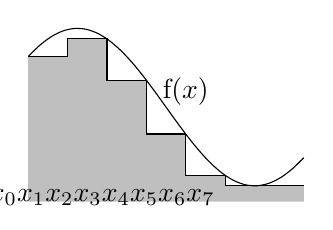
\begin{tikzpicture}
  
\path[fill=lightgray]
	(0.5, 1.84279) -| (1, 2.06603) -| (1.5, 1.54202) -| (2, 0.85798) -| (2.5, 0.33397) -| (3, 0.2) -| (4, 0.2) --
	(4, 0) -- (0.5, 0) -- (0.5, 1.84279);

\draw (0.5, 1.84279) -| (1, 2.06603) -| (1.5, 1.54202) -| (2, 0.85798) -| (2.5, 0.33397) -| (3, 0.2) -| (4, 0.2);

\draw [smooth, domain=0.5:4] plot({\x}, {1.2 + sin(80 * \x)});
\draw (2.5, 1.4) node{\(\mathrm{f}(x)\)};

\drawaxesxy{0}{0}{-0.5}{-0.5}{4.5}{2.5}

\drawxcoord{0.5}{0}{\(x_0\)}
\drawxcoord{1}{0}{\(x_1\)}
\drawxcoord{1.5}{0}{\(x_2\)}
\drawxcoord{2}{0}{\(x_3\)}
\drawxcoord{2.5}{0}{\(x_4\)}
\drawxcoord{3}{0}{\(x_5\)}
\drawxcoord{3.5}{0}{\(x_6\)}
\drawxcoord{4}{0}{\(x_7\)}

\end{tikzpicture}
\caption{Dolní mez integtrálu}
\end{center}
\label{img:integral_dolni_mez}
\end{figure}

Horní mez integrálu je dána vztahem

\begin{equation}
\label{eq:horni_mez_integralu}
\overline{\int}_a^b \mathrm{f}(x) \cdot \mathrm{d}x = \sum_{i} (x_{i+1} - x_i) \cdot \max(\{\mathrm{f}(x) | x_i \leq x \leq x_{i+1}\})
\end{equation}

a~její grafická interpretace je vidět na obrázku~\ref{img:integral_horni_mez}.

\begin{figure}[ht]
\begin{center}
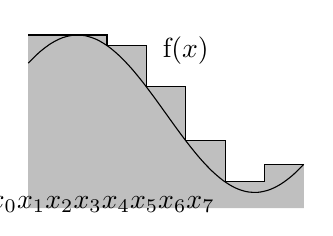
\begin{tikzpicture}
  
\path[fill=lightgray]
	(0.5, 2.2) -| (1.5, 2.06603) -| (2, 1.54202) -| (2.5, 0.85798) -| (3, 0.33397) -| (3.5, 0.55721) -| (4, 0.55721) --
	(4, 0) -- (0.5, 0) -- (0.5, 2.2);

\draw (0.5, 2.2) -| (1.5, 2.06603) -| (2, 1.54202) -| (2.5, 0.85798) -| (3, 0.33397) -| (3.5, 0.55721) -| (4, 0.55721);

\draw [smooth, domain=0.5:4] plot({\x}, {1.2 + sin(80 * \x)});
\draw (2.5, 2) node{\(\mathrm{f}(x)\)};

\drawaxesxy{0}{0}{-0.5}{-0.5}{4.5}{2.5}

\drawxcoord{0.5}{0}{\(x_0\)}
\drawxcoord{1}{0}{\(x_1\)}
\drawxcoord{1.5}{0}{\(x_2\)}
\drawxcoord{2}{0}{\(x_3\)}
\drawxcoord{2.5}{0}{\(x_4\)}
\drawxcoord{3}{0}{\(x_5\)}
\drawxcoord{3.5}{0}{\(x_6\)}
\drawxcoord{4}{0}{\(x_7\)}

\end{tikzpicture}
\caption{Horní mez integrálu}
\end{center}
\label{img:integral_horni_mez}
\end{figure}

Dělení intervalu nemusí být rovnoměrné. Označme toto dělení \(d\) a~nejdelší interval tohoto dělení \(\delta_d = \max(x_{i+1} - x_i)\). Pak můžeme spočítat limity dolních a~horních mezí. Povšimněme si, že dělení intervalu není určeno jednoznačně a~my v~limitách bereme v~potaz nejhorší případ. Pokud platí

\begin{equation}
\lim_{\delta_m \to 0} \max \left(\left\{\overline{\int}_a^b \mathrm{f}(x) \cdot \mathrm{d}x - \underline{\int}_a^b \mathrm{f}(x) \cdot \mathrm{d}x \middle| \delta_d \leq \delta_m \right\}\right) = 0
\end{equation}

tedy pokud rozdíl a~dolní meze konverguje k~nule, pak jsou tyto limity rovny integrálu:

\begin{equation}
\begin{split}
\int_a^b \mathrm{f}(x) \cdot \mathrm{d}x = \\
\lim_{\delta_m \to 0} \min \left(\left\{\underline{\int}_a^b \mathrm{f}(x) \cdot \mathrm{d}x \middle| \delta_d \leq \delta_m \right\}\right) = \\
\lim_{\delta_m \to 0} \max \left(\left\{\overline{\int}_a^b \mathrm{f}(x) \cdot \mathrm{d}x \middle| \delta_d \leq \delta_m \right\}\right)
\end{split}
\end{equation}

To tedy znamená, že k~integrálu bude konvergovat i~každá posloupnost, která vznikne tak, že sečteme libovolné body z~intervalů vzniklých dělením. Je tomu tak proto, že tyto body budou ležet mezi minimi a~maximy těchto intervalů:

\begin{equation}
\label{eq:vypocet_integralu}
\int_a^b \mathrm{f}(x) \cdot \mathrm{d}x = \lim_{\delta_m \to 0} \sum_{i} (x_{i+1} - x_i) \cdot \mathrm{f}(x_i \leq x \leq x_{i+1})
\end{equation}

Prozkoumejme existenci integrálu. Nechť je funkce \(\mathrm{f}(x)\) spojitá na intervalu \(<a; b>\), to tedy předpokládá, že funkce má na celém intervalu limitu. Z~definice limity tedy musí pro každý bod existovat (obecně různá) funkce \(\delta(\varepsilon)\). Nechť \(\delta_{inf}(\varepsilon)\) označuje její infimum přes všechny body intervalu. Potom pro jakýkoli interval \(<x_i; x_{i+1}>\), kde \(x_{i+1} - x_i < \delta_{inf}(\varepsilon)\), musí platit 

\begin{equation}
\max(\{\mathrm{f}(x) | x_i \leq x \leq x_{i+1}\}) - \min(\{\mathrm{f}(x) | x_i \leq x \leq x_{i+1}\}) < \varepsilon
\end{equation}

Je tomu tak proto, že \(\delta_{inf}\)-okolí jakéhokoli bodu intervalu je celý interval. Proto pro každé dostatečně jemné dělení intervalu bude platit

\begin{equation}
\begin{split}
\lim_{\delta_m \to 0} \left( \overline{\int}_a^b \mathrm{f}(x) \cdot \mathrm{d}x - \underline{\int}_a^b \mathrm{f}(x) \cdot \mathrm{d}x \right) = \\
\lim_{\delta_m \to 0} \Bigg( \sum_{i} (x_{i+1} - x_i) \cdot \max(\{\mathrm{f}(x) | x_i \leq x \leq x_{i+1}\}) - \\
\sum_{i} (x_{i+1} - x_i) \cdot \min(\{\mathrm{f}(x) | x_i \leq x \leq x_{i+1}\}) \Bigg) = \\
\lim_{\delta_m \to 0} \Bigg( \sum_{i} (x_{i+1} - x_i) \cdot (\max(\{\mathrm{f}(x) | x_i \leq x \leq x_{i+1}\}) - \\
\min(\{\mathrm{f}(x) | x_i \leq x \leq x_{i+1}\})) \Bigg) = \\
\sum_{i} (x_{i+1} - x_i) \cdot \lim_{\delta_m \to 0} (\max(\{\mathrm{f}(x) | x_i \leq x \leq x_{i+1}\}) - \\
\min(\{\mathrm{f}(x) | x_i \leq x \leq x_{i+1}\})) = 0
\end{split}
\end{equation}

Proto každá spojitá funkce má integrál. Zvažme dále, co se stane, pokud by funkce nebyla spojitá v~konečném počtu \(n\) bodů. Z~integrálu tyto body vyjmeme. Prozkoumejme, co se stane se sumou ve vztahu~\eqref{eq:dolni_mez_integralu} respektive~\eqref{eq:horni_mez_integralu}. Každý z~vyňatých bodů může být v~nejhorším případě obsažen ve dvou intervalech (pokud by ležel na jejich hranici). Jejich součet v~uvedených sumách je proto v~limitě

\begin{equation}
\lim_{\delta_m \to 0} 2 \cdot n \cdot \delta_m \cdot x = 0 
\end{equation}

a~integrál proto neovlivní. Z~toho plynou závěry:

\begin{fact}
Každá po částech spojitá funkce má integrál.
\end{fact}

\begin{fact}
Odebráním konečného počtu bodů z~integrované funkce se integrál nezmění.
\end{fact}

Vraťme se ještě k~rovnici \eqref{eq:scitani_integralu} a~zapišme ji s~jiným označením mezí: 

\begin{equation}
\begin{split}
\int_{x_0}^{b} \mathrm{f}(x) \cdot \mathrm{d}x = \int_{x_0}^{a} \mathrm{f}(x) \cdot \mathrm{d}x + \int_{a}^{b} \mathrm{f}(x) \cdot \mathrm{d}x \\
\int_{a}^{b} \mathrm{f}(x) \cdot \mathrm{d}x = \int_{x_0}^{b} \mathrm{f}(x) \cdot \mathrm{d}x - \int_{x_0}^{a} \mathrm{f}(x) \cdot \mathrm{d}x
\end{split}
\end{equation}

Zavedeme-li pro libovolně zvolenou hodnotu \(x_0\) tzv. primitivní funkci

\begin{equation}
\mathrm{F}(x) = \int_{x_0}^{x} \mathrm{f}(x) \cdot \mathrm{d}x
\end{equation}

pak můžeme rovnici přepsat do tvaru:

\begin{equation}
\label{eq:vztah_mezi_neurcitym_a_urcitym_integralem}
\int_{a}^{b} \mathrm{f}(x) \cdot \mathrm{d}x = \mathrm{F}(b) - \mathrm{F}(a) = \left[\mathrm{F}(x)\right]_a^b 
\end{equation}

Primitivní funkce budeme zapisovat velkými písmeny.
Označením \(\left[\mathrm{F}(x)\right]_a^b\) myslíme právě výraz \(\mathrm{F}(b) - \mathrm{F}(a)\), tedy rozdíl hodnot výrazu v~závorce vyhodnoceného pro \(b\) a~\(a\).

Povšimněme si, že primitivní funkce není určena jednoznačně. Můžeme k~ní pripočíst libovolnou konstantu a~rozdíl ve vztahu~\eqref{eq:vztah_mezi_neurcitym_a_urcitym_integralem} to nijak neovlivní. Množinu všech primitivních funkcí lišících se o~konstantu nazýváme neurčitý integrál a~píšeme ho ve tvaru:

\begin{equation}
\int \mathrm{f}(x) \cdot \mathrm{d}x = \mathrm{F}(x) + \mathrm{C}
\end{equation}

Naproti tomu integrál \(\int_a^b \mathrm{f}(x) \cdot \mathrm{d}x\) nazýváme určitý integrál.

Zkusme vyjádřit, jak se primitivní funkce chová v~okolí bodu:

\begin{equation}
\begin{split}
\mathrm{F}(x + \mathrm{d}x) = \int_{x_0}^{x + \mathrm{d}x} \mathrm{f}(x) \cdot \mathrm{d}x = \int_{x_0}^{x} \mathrm{f}(x) \cdot \mathrm{d}x + \int_{x}^{x + \mathrm{d}x} \mathrm{f}(x) \cdot \mathrm{d}x = \\
\mathrm{F}(x) + \int_{x}^{x + \mathrm{d}x} \mathrm{f}(x) \cdot \mathrm{d}x
\end{split}
\end{equation}

Protože \(\mathrm{d}x\) je nekonečně malý, tak můžeme funkci \(\mathrm{f}(x)\) považovat mezi \(x\) a~\(x + \mathrm{f}(x)\) za konstantní. Přesněji, \(\mathrm{d}x\) je tak malé, že interval \(<x; x + \mathrm{d}x>\) je rozdělen pouze na jeden podinterval. Suma ve vztahu~\eqref{eq:vypocet_integralu} proto přejde do tvaru \(\mathrm{d}x \cdot \mathrm{f}(x)\).
Proto platí:

\begin{equation}
\begin{split}
\mathrm{F}(x + \mathrm{d}x) = \mathrm{F}(x) + \mathrm{f}(x) \cdot \mathrm{d}x \\
\mathrm{f}(x) = \lim_{\mathrm{d}x \to 0} \frac{\mathrm{F}(x + \mathrm{d}x) - \mathrm{F}(x)}{\mathrm{d}x} = \frac{\partial \mathrm{F}}{\partial x} 
\end{split}
\end{equation}

Vidíme tedy, že derivování je opačná operace než integrování. Tento fakt se nazývá fundamentální věta matematické analýzy:

\begin{fact}
\begin{equation}
\mathrm{f}(x) = \frac{\partial \mathrm{F}}{\partial x} \Leftrightarrow \int \mathrm{f}(x) \cdot \mathrm{d}x = \mathrm{F}(x) + \mathrm{C}
\end{equation}
\end{fact}

Takto můžeme vyjádřit integrály k~elementárním funkcím. Vyjádřeny jsou v~příloze~\ref{ap:integraly_zakladnich_funkci}.

\section{Integrování pomocí substituce}

Začněme vztahem pro derivování složené funkce, přičemž platí \(\mathrm{f}(t) = \frac{\partial \mathrm{F}}{\partial t}\):

\begin{equation}
\frac{\partial}{\partial x} \mathrm{F}(\mathrm{g}(x)) = \frac{\partial \mathrm{F}}{\partial x} (\mathrm{g}(x)) \cdot \frac{\partial \mathrm{g}}{\partial x} = \mathrm{f}(\mathrm{g}(x)) \cdot \frac{\partial \mathrm{g}}{\partial x}
\end{equation}

Obě strany rovnice zintegrujeme

\begin{equation}
\mathrm{F}(\mathrm{g}(x)) = \int \mathrm{f}(\mathrm{g}(x)) \cdot \frac{\partial \mathrm{g}}{\partial x} \cdot \mathrm{d}x
\end{equation}

a~můžeme zavést substituci \(t = \mathrm{g}(x)\): 

\begin{equation}
\int \mathrm{f}(\mathrm{g}(x)) \cdot \frac{\partial \mathrm{g}}{\partial x} \cdot \mathrm{d}x = \mathrm{F}(t) = \int \mathrm{f}(t) \cdot \mathrm{d}t
\end{equation}

Integrovat pomocí substituce můžeme přímo i~určité integrály.

\begin{equation}
\int_a^b \mathrm{f}(\mathrm{g}(x)) \cdot \frac{\partial \mathrm{g}}{\partial x} \cdot \mathrm{d}x = [\mathrm{F}(\mathrm{g}(x))]_a^b = [\mathrm{F}(t)]_{\mathrm{g}(a)}^{\mathrm{g}(b)} = \int_{\mathrm{g}(a)}^{\mathrm{g}(b)} \mathrm{f}(t) \cdot \mathrm{d}t
\end{equation}

\begin{fact}
\begin{equation}
\int \mathrm{f}(\mathrm{g}(x)) \cdot \frac{\partial \mathrm{g}}{\partial x} \cdot \mathrm{d}x = \int \mathrm{f}(t) \cdot \mathrm{d}t; t = \mathrm{g}(x)
\end{equation}

\begin{equation}
\int_a^b \mathrm{f}(\mathrm{g}(x)) \cdot \frac{\partial \mathrm{g}}{\partial x} \cdot \mathrm{d}x = \int_{\mathrm{g}(a)}^{\mathrm{g}(b)} \mathrm{f}(t) \cdot \mathrm{d}t
\end{equation}

\end{fact}

\section{Integrování per partes}

Vyjděme ze vztahu pro derivaci součinu:

\begin{equation}
\frac{\partial}{\partial x} (\mathrm{f}(x) \cdot \mathrm{g}(x)) = \mathrm{g}(x) \cdot \frac{\partial \mathrm{f}}{\partial x} + \mathrm{f}(x) \cdot \frac{\partial \mathrm{g}}{\partial x}
\end{equation}

Aplikujeme fundamentální větu matematické analýzy a~přeuspořádáme výraz:

\begin{equation}
\begin{split}
\mathrm{f}(x) \cdot \mathrm{g}(x) = \int \mathrm{g}(x) \cdot \frac{\partial \mathrm{f}}{\partial x} \cdot \mathrm{d}x + \int \mathrm{f}(x) \cdot \frac{\partial \mathrm{g}}{\partial x} \cdot \mathrm{d}x \\
\int \mathrm{f}(x) \cdot \frac{\partial \mathrm{g}}{\partial x} \cdot \mathrm{d}x = \mathrm{f}(x) \cdot \mathrm{g}(x) - \int \mathrm{g}(x) \cdot \frac{\partial \mathrm{f}}{\partial x} \cdot \mathrm{d}x
\end{split}
\end{equation}

Vztah můžeme vyjádřit i~pro určitý integrál:

\begin{equation}
\begin{split}
\int_a^b \mathrm{f}(x) \cdot \frac{\partial \mathrm{g}}{\partial x} \cdot \mathrm{d}x = \left[ \int \mathrm{f}(x) \cdot \frac{\partial \mathrm{g}}{\partial x} \cdot \mathrm{d}x \right]_a^b = \\
\left[ \mathrm{f}(x) \cdot \mathrm{g}(x) - \int \mathrm{g}(x) \cdot \frac{\partial \mathrm{f}}{\partial x} \cdot \mathrm{d}x \right]_a^b = \\
\left[ \mathrm{f}(x) \cdot \mathrm{g}(x) \right]_a^b - \int_a^b \mathrm{g}(x) \cdot \frac{\partial \mathrm{f}}{\partial x} \cdot \mathrm{d}x
\end{split}
\end{equation}

\begin{fact}
\begin{equation}
\int \mathrm{f}(x) \cdot \frac{\partial \mathrm{g}}{\partial x} \cdot \mathrm{d}x = \mathrm{f}(x) \cdot \mathrm{g}(x) - \int \mathrm{g}(x) \cdot \frac{\partial \mathrm{f}}{\partial x} \cdot \mathrm{d}x
\end{equation}

\begin{equation}
\int_a^b \mathrm{f}(x) \cdot \frac{\partial \mathrm{g}}{\partial x} \cdot \mathrm{d}x =
\left[ \mathrm{f}(x) \cdot \mathrm{g}(x) \right]_a^b - \int_a^b \mathrm{g}(x) \cdot \frac{\partial \mathrm{f}}{\partial x} \cdot \mathrm{d}x
\end{equation}
\end{fact}

\section{Vícerozměrný integrál}

Doposud jsme pracovali s~jednorozměrným integrálem - definičním oborem integrované funkce byl (pod)množina reálných čísel. Určitý integrál jsme definovali jako plochu pod křivkou určenou funkcí s~jedním parametrem probíhajícím po určitém intervalu. Tuto definici můžeme rozšířit na funkci se dvěma parametry probíhajícími po obdélníku, se třemi parametry probíhajícími po kvádru nebo obecně s~více parametry probíhajícími po hyperkvádru.

Mějme funkci s~více parametry \(\mathrm{f}(x, y, ...)\), kterou budeme integrovat obecně na hyperkvádru \(\Omega\) se stranamy \(<a_x; b_x>\), \(<a_y; b_y>\) atd. Tyto strany rozdělíme na konečný počet intervalů \(<x_0, x_1>\), \(<x_1, x_2>\), ...,  \(<y_0, y_1>\), \(<y_1, y_2>\) atd. Tím vznikne mřížka dělící hyperkvádr \(\Omega\) na malé hyperkvádry. Dolní mez integrálu je pak dána vztahem

\begin{equation}
\label{eq:dolni_mez_vicerozmerneho_integralu}
\underline{\int_{\Omega}} \mathrm{f}(x, y, ...) \cdot \mathrm{d}V = \sum_{i, j, ...} (x_{i+1} - x_i) \cdot (y_{j+1} - y_j) \cdot ... \cdot \min_{i, j, ..}(\mathrm{f})
\end{equation}

přičemž zápisem \(\min_{i, j, ..}(\mathrm{f})\) rozumíme minimální hodnotu funkce \(\mathrm{f}\) na malém hyperkvádru:

\begin{equation}
\min_{i, j, ..}(\mathrm{f}) = \min(\{\mathrm{f}(x, y, ...) | x_i \leq x \leq x_{i+1} \land y_j \leq y \leq y_{j+1} \land ...\})
\end{equation}

Horní mez integrálu je obdobně dána vztahem

\begin{equation}
\label{eq:horni_mez_vicerozmerneho_integralu}
\overline{\int_{\Omega}} \mathrm{f}(x, y, ...) \cdot \mathrm{d}V = \sum_{i, j, ...} (x_{i+1} - x_i) \cdot (y_{j+1} - y_j) \cdot ... \cdot \max_{i, j, ..}(\mathrm{f})
\end{equation}

přičemž zápisem \(\max_{i, j, ..}(\mathrm{f})\) rozumíme maximální hodnotu funkce \(\mathrm{f}\) na malém hyperkvádru:

\begin{equation}
\max_{i, j, ..}(\mathrm{f}) = \max(\{\mathrm{f}(x, y, ...) | x_i \leq x \leq x_{i+1} \land y_j \leq y \leq y_{j+1} \land ...\})
\end{equation}

Dělení hyperkvádru \(\Omega\) nemusí být rovnoměrné. Označme toto dělení \(d\) a~nejdelší interval jakéhokoli parametru tohoto dělení \(\delta_d = \max(x_{i+1} - x_i, y_{i+1} - y_i, ...)\). Pak můžeme obdobně jako u~jednorozměrného integrálu spočítat limity dolních a~horních mezí. Pokud platí

\begin{equation}
\lim_{\delta_m \to 0} \max \left(\left\{\overline{\int_{\Omega}} \mathrm{f}(x) \cdot \mathrm{d}V - \underline{\int_{\Omega}} \mathrm{f}(x) \cdot \mathrm{d}V \middle| \delta_d \leq \delta_m \right\}\right) = 0
\end{equation}

tedy pokud rozdíl a~dolní meze konverguje k~nule, pak jsou tyto limity rovny integrálu:

\begin{equation}
\begin{split}
\int_{\Omega} \mathrm{f}(x) \cdot \mathrm{d}V = \\
\lim_{\delta_m \to 0} \min \left(\left\{\underline{\int_{\Omega}} \mathrm{f}(x) \cdot \mathrm{d}V \middle| \delta_d \leq \delta_m \right\}\right) = \\
\lim_{\delta_m \to 0} \max \left(\left\{\overline{\int_{\Omega}} \mathrm{f}(x) \cdot \mathrm{d}V \middle| \delta_d \leq \delta_m \right\}\right)
\end{split}
\end{equation}

To tedy znamená, že k~integrálu bude konvergovat i~každá posloupnost, která vznikne tak, že sečteme libovolné body z~hyperkvádrům vzniklých dělením. Je tomu tak proto, že tyto body budou ležet mezi minimi a~maximy těchto hyperkvádrů:

\begin{equation}
\begin{split}
\int_{\Omega} \mathrm{f}(x) \cdot \mathrm{d}V = \\
\lim_{\delta_m \to 0} \sum_{i} (x_{i+1} - x_i) \cdot y_{j+1} - y_j) \cdot ... \cdot \mathrm{f}(x_i \leq x \leq x_{i+1}, y_j \leq y \leq y_{j+1}, ...)
\end{split}
\end{equation}

Prozkoumejme existenci integrálu. Nechť je funkce \(\mathrm{f}(x, y, ...)\) spojitá na hyperkvádru \(\Omega\), to tedy předpokládá, že funkce zde má limitu. Z~definice limity tedy musí pro každý bod existovat (obecně různá) funkce \(\delta(\varepsilon)\). Označme \(\delta_{inf}(\varepsilon)\) její infimum přes všechny body. Dva body ležící v~\(n\)-rozměrném hyperkvádru se všemi hranami o~délce nejvýše \(\delta\) mohou mít vzdálenost nejvýše \(\sqrt{n} \cdot \delta\). Proto pokud \(\delta_d \leq \frac{\delta_{inf}(\epsilon)}{\sqrt{n}}\), pak musí platit: 

\begin{equation}
\max(\{\mathrm{f}(x) | x_i \leq x \leq x_{i+1}\}) - \min(\{\mathrm{f}(x) | x_i \leq x \leq x_{i+1}\}) < \varepsilon
\end{equation}

Je tomu tak proto, že \(\delta_{inf}\)-okolí jakéhokoli bodu intervalu obsahuje celý hyperkvádr vzniklý dělením. Proto pro každé dostatečně jemné dělení intervalu bude platit

\begin{equation}
\begin{split}
\lim_{\delta_m \to 0} \left( \overline{\int_{\Omega}} \mathrm{f}(x) \cdot \mathrm{d}x - \underline{\int_{\Omega}} \mathrm{f}(x) \cdot \mathrm{d}x \right) = \\
\lim_{\delta_m \to 0} \Bigg( \sum_{i} (x_{i+1} - x_i) \cdot \max_{i, j, ..}(\mathrm{f}) -
\sum_{i} (x_{i+1} - x_i) \cdot \min_{i, j, ..}(\mathrm{f}) \Bigg) = \\
\lim_{\delta_m \to 0} \Bigg( \sum_{i} (x_{i+1} - x_i) \cdot (\max_{i, j, ..}(\mathrm{f}) -
\min_{i, j, ..}(\mathrm{f}) \Bigg) = \\
\sum_{i} (x_{i+1} - x_i) \cdot \lim_{\delta_m \to 0} (\max_{i, j, ..}(\mathrm{f}) -
\min_{i, j, ..}(\mathrm{f})) = 0
\end{split}
\end{equation}

Proto každá spojitá funkce má integrál. Zvažme dále, co se stane, pokud by funkce nebyla spojitá v~konečném počtu hladkých \(n-1\) rozměrných hyperploch. Z~integrálu tyto hyperploch vyjmeme. Prozkoumejme, co se stane se sumou ve vztahu~\eqref{eq:dolni_mez_vicerozmerneho_integralu} respektive~\eqref{eq:horni_mez_vicerozmerneho_integralu}. Každá z~vyňatých hyperploch může být v~nejhorším případě obsažena \(\frac{C}{\delta_m^{n-1}}\) hyperkvádrů. Jejich součet v~uvedených sumách je proto v~limitě

\begin{equation}
\lim_{\delta_m \to 0} \frac{C}{\delta_m^{n-1}} \cdot \delta_m^n \cdot x = \lim_{\delta_m \to 0} C \cdot \delta_m \cdot x = 0 
\end{equation}

a~integrál proto neovlivní. Z~toho plynou závěry:

\begin{fact}
Každá funkce spojitá až na konečný počet hladkých \(n-1\) rozměrných hyperploch má \(n\)-rozměrný integrál.
\end{fact}

\begin{fact}
Odebráním bodů ležících na konečném počtu hladkých \(n-1\) rozměrných hyperplochách z~integrované funkce se integrál nezmění.
\end{fact}


\section{Křivkový integrál}

Pokud máme orientovanou po částech hladkou křivku v~prostoru definovanou parametricky pomocí rovnice \eqref{eq:krivkovy_integral_krivka} a~kovariantní vektorové pole \(\kovarvect{v}\), pak křivkový integrál definujeme rovnicí \eqref{eq:krivkovy_integral_definice}.

\begin{equation}
\label{eq:krivkovy_integral_krivka}
\Gamma = (\Gamma^1(t), \Gamma^2(t), ..., \Gamma^n(t)), t \in <t_1, t_2>
\end{equation}

\begin{equation}
\label{eq:krivkovy_integral_definice}
\begin{split}
\int_\Gamma \kovarvect{v} \cdot d\kontravect{l}
\end{split}
\end{equation}

Protože \(\frac{d\kontravect{l}}{dt} = \left(\frac{d \Gamma^1}{dt}, \frac{d \Gamma^2}{dt}, ..., \frac{d \Gamma^n}{dt} \right)\), tak pro parametrickou křivku
\(\Gamma\) platí vztah \eqref{eq:krivkovy_integral_vypocet}.

\begin{equation}
\label{eq:krivkovy_integral_vypocet}
\begin{split}
\int_\Gamma \kovarvect{v} \cdot d\kontravect{l} =
\int_{t_1}^{t_2} \left(\sum_{i=1}^n v_i(\Gamma(t)) \cdot \frac{d \Gamma^i}{dt} \right) dt
\end{split}
\end{equation}

Vidíme, proč vektorové pole \(\kovarvect{v}\) musí být kovariantní. Protože diferenciály souřadnic křivky tvoří kontravariantní vektor, tak pole \(\kovarvect{v}\) musí být kovariantní, aby jejich skalární součin byl invariantní vůči změně soustavy souřadnic. Křivkový integrál je proto také invariantní vůči změně soustavy souřadnic.

Je-li křivka uzavřená (její počáteční a koncový bod jsou shodné), toto zdůrazníme kroužkem přes symbol integrálu, tedy \(\oint_\Gamma \kovarvect{v} \cdot d\kontravect{l}\), a říkáme mu cirkulace vektoru po uzavřené smyčce.

Z definice \eqref{eq:krivkovy_integral_definice} plyne, že integrujeme skalární součin hodnoty pole \(v\) a elementu dráhy \(dl\),
tedy součin průmětu pole do dráhy a elementu dráhy. Křivkový integrál proto lze použít pro výpočet práce, energie a podobně.


\subsection{Příklad}

Elektrické pole má intenzitu \(E = \left(-\frac{y}{x^2+y^2}, \frac{x}{x^2+y^2}\right) \frac{\mathrm{N}}{\mathrm{C}}\). Jakou práci pole vykoná na jednotkovém náboji, který se pohybuje po dráze \(\Gamma(t) = (1, t), t \in <-1, 1>\)?


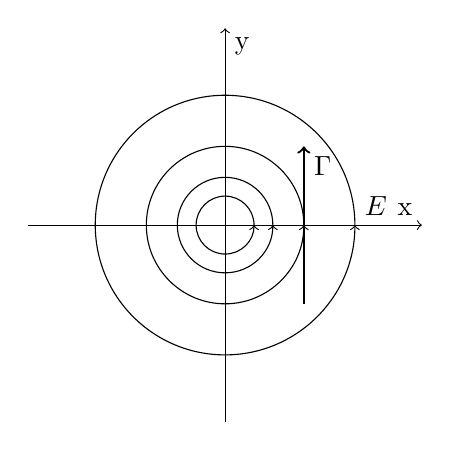
\begin{tikzpicture}
\draw[->] (-2.5, 0) -- (2.5, 0) node[anchor=south east]{x};
\draw[->] (0, -2.5) -- (0, 2.5) node[anchor=north west]{y};

\foreach \r in {0.3679, 0.6065, 1, 1.6487}
	\draw[->, thin] (\r, 0) arc (0:360:\r);
	
\draw (1.65, 0) node[anchor=south west]{\(\vect{E}\)};
	
\draw[->, thick] (1, -1) -- (1, 1) node[anchor=north west]{\(\Gamma\)};
\end{tikzpicture}


Elektrické pole působí na náboj \(Q\) silou \(\vect{F} = \vect{E} \cdot Q\). Práce vykonaná přesunutím náboje \(Q\) po dráze \(\vect{ds}\) je tedy \(dW = \vect{F} \cdot \vect{ds} = \vect{E} \cdot Q \cdot \vect{ds}\) a pro jednotkový náboj \(dW = \vect{E} \cdot \vect{ds}\). Celková práce je tedy

\[
W = \int_{-1}^1 \left (\frac{-t}{1 + t^2} \cdot 0 + \frac{1}{1 + t^2} \cdot 1 \right) = \left[\mathrm{arctg} \ t\right]_{-1}^1 = \frac{\pi}{2} \mathrm{J}
\]

\subsection{Vlastnosti křivkového integrálu}

Nyní vyšetřeme vlastnosti křivkového integrálu. Rovnice \eqref{eq:krivkovy_integral_linearita} udává linearitu křivkového integrálu. Rovnice \eqref{eq:krivkovy_integral_opacny} říká, že křivkový integrál po opačně orientované křivce je opačný. Rovnice \eqref{eq:krivkovy_integral_soucet} udává, že křivkový integrál po křivce, která je rovna součtu dvou křivek, je rovna součtu jejich křivkových integrálů. Oba dva vztahy jsou intuitivní a~lze je snadno ověřit rozepsáním integrálů pomocí vztahu \eqref{eq:krivkovy_integral_vypocet}.

\begin{equation}
\label{eq:krivkovy_integral_linearita}
\begin{split}
\int_{\Gamma} \left(\alpha \kovarvect{u} + \beta \kovarvect{v}\right) \cdot d\kontravect{l} = \alpha \int_{\Gamma} \kovarvect{u} \cdot d\kontravect{l} + \beta \int_{\Gamma} \kovarvect{v} \cdot d\kontravect{l}
\end{split}
\end{equation}

\begin{equation}
\label{eq:krivkovy_integral_opacny}
\begin{split}
\int_{-\Gamma} \kovarvect{v} \cdot d\kontravect{l} = -\int_{\Gamma} \kovarvect{v} \cdot d\kontravect{l}
\end{split}
\end{equation}

\begin{equation}
\label{eq:krivkovy_integral_soucet}
\begin{split}
\int_{\Gamma_1 + \Gamma_2} \kovarvect{v} \cdot d\kontravect{l} = \int_{\Gamma_1} \kovarvect{v} \cdot d\kontravect{l} + \int_{\Gamma_2} \kovarvect{v} \cdot d\kontravect{l}
\end{split}
\end{equation}

Protože skalární součin nezávisí na volbě soustavy souřadnic, tak ani křivkový integrál definovaný vztahem \eqref{eq:krivkovy_integral_definice} nezávisí na volbě soustavy souřadnic. Pro stejné pole a pro stejnou křivku bude křivkový integrál stejný. Je to patrné i z fyzikálního významu. Pokud bude křivkový integrál představovat celkovou práci, pak ta nezávisí na volbě soustavy souřadnic.

Máme-li uzavřenou smyčku \(\Gamma_S\), pak ji můžeme rozdělit na dvě smyčky \(\Gamma_1\) a~\(\Gamma_2\) pomocí libovolně volené přepážky \(\Gamma_P\).

\begin{tikzpicture}
\tikzmath{ \x = 0; \y = 5; }

\draw[->] (\x + 2, \y) arc (0:360:2 and 1);
\draw (\x + 2, \y) node[anchor=west]{\(\Gamma_S\)};

\tikzmath{ \x = 0; \y = 2.5; \t = 0.1; }

\draw[->] (\x + \t, \y - 1) arc (-90:90:2 and 1);
\draw[->] (\x + \t, \y + 1) -- (\x + \t, \y - 0.9);

\draw[->] (\x - \t, \y + 1) arc (90:270:2 and 1);
\draw[->] (\x - \t, \y - 0.9) -- (\x - \t, \y + 1);
\draw (\x, \y) node[anchor=west]{\(\Gamma_P\)};

\draw (\x + \t, \y - 0.9) -- (\x - \t, \y - 0.9);
\draw (\x - \t, \y - 1) -- (\x + \t, \y - 1);

\tikzmath{ \x = 0; \y = 0; \t = 0.1; }

\draw[->] (\x + \t, \y - 1) arc (-90:90:2 and 1);
\draw[->] (\x + \t, \y + 1) -- (\x + \t, \y - 1);
\draw (\x - 2, \y + 0) node[anchor=east]{\(\Gamma_1\)};

\draw[->] (\x - \t, \y + 1) arc (90:270:2 and 1);
\draw[->] (\x - \t, \y - 1) -- (\x - \t, \y + 1);
\draw (\x + 2, \y) node[anchor=west]{\(\Gamma_2\)};
\end{tikzpicture}

Přepážka je tvořena dvěma opačně orientovanými částmi křivky, které jsou nekonečně blízké. Proto se jejich příspěvky do cirkulace vyruší a platí proto vztah \eqref{eq:deleni_cirkulace}. Takto lze cirkulaci vektoru podél křivky rozdělit na součet libovolného počtu cirkulací.

\begin{equation}
\label{eq:deleni_cirkulace}
\begin{split}
\oint_{\Gamma_S} \kovarvect{v} \cdot d\kontravect{l} = \oint_{\Gamma_1} \kovarvect{v} \cdot d\kontravect{l} + \oint_{\Gamma_2} \kovarvect{v} \cdot d\kontravect{l}
\end{split}
\end{equation}

\subsection{Rotace}
\label{sec:rotace}

Vyšetřeme nyní cirkulaci vektoru nekonečně malou smyčkou. Vektorové pole \(\vect{v}\) linearizujeme podle vztahu \eqref{eq:rotace_linearizace}.
Předpokládáme, že pole pole je hladké - má derivace prvního řádu.

\begin{equation}
\label{eq:rotace_linearizace}
\vect{v} \approx \begin{pmatrix}
v_{x_0} + \frac{\partial v_x}{\partial x} \cdot x + \frac{\partial v_x}{\partial y} \cdot y + \frac{\partial v_x}{\partial z} \cdot z \\
v_{y_0} + \frac{\partial v_y}{\partial x} \cdot x + \frac{\partial v_y}{\partial y} \cdot y + \frac{\partial v_y}{\partial z} \cdot z \\
v_{z_0} + \frac{\partial v_z}{\partial x} \cdot x + \frac{\partial v_z}{\partial y} \cdot y + \frac{\partial v_z}{\partial z} \cdot z
\end{pmatrix}
\end{equation}

Dosadíme-li linearizaci \eqref{eq:rotace_linearizace} do vztahu \eqref{eq:krivkovy_integral_vypocet}, získáme vztah \eqref{eq:rotace_1}.

\begin{equation}
\label{eq:rotace_1}
\int_\Gamma \vect{v} \cdot d\vect{l} \approx
\int_{t_1}^{t_2} \begin{pmatrix}
\left(v_{x_0} + \frac{\partial v_x}{\partial x} \cdot \Gamma_x(t) + \frac{\partial v_x}{\partial y} \cdot \Gamma_y(t) + \frac{\partial v_x}{\partial z} \cdot \Gamma_z(t)\right) \cdot \frac{d \Gamma_x}{dt} + \\
\left(v_{y_0} + \frac{\partial v_y}{\partial x} \cdot \Gamma_x(t) + \frac{\partial v_y}{\partial y} \cdot \Gamma_y(t) + \frac{\partial v_y}{\partial z} \cdot \Gamma_z(t)\right) \cdot \frac{d \Gamma_y}{dt} + \\
\left(v_{z_0} + \frac{\partial v_z}{\partial x} \cdot \Gamma_x(t) + \frac{\partial v_z}{\partial y} \cdot \Gamma_y(t) + \frac{\partial v_z}{\partial z} \cdot \Gamma_z(t)\right) \cdot \frac{d \Gamma_z}{dt}
\end{pmatrix} dt
\end{equation}

Úpravou získáme vztah \eqref{eq:rotace_2}.

\begin{equation}
\label{eq:rotace_2}
\begin{matrix}
v_{x_0} \int_{t_1}^{t_2} \frac{d \Gamma_x}{dt} dt + \frac{\partial v_x}{\partial x} \int_{t_1}^{t_2} \Gamma_x(t) \frac{d \Gamma_x}{dt} dt + \frac{\partial v_x}{\partial y} \int_{t_1}^{t_2} \Gamma_y(t) \frac{d \Gamma_x}{dt} dt + \frac{\partial v_x}{\partial z} \int_{t_1}^{t_2} \Gamma_z(t) \frac{d \Gamma_x}{dt} dt + \\
v_{y_0} \int_{t_1}^{t_2} \frac{d \Gamma_y}{dt} dt + \frac{\partial v_y}{\partial x} \int_{t_1}^{t_2} \Gamma_x(t) \frac{d \Gamma_y}{dt} dt + \frac{\partial v_y}{\partial y} \int_{t_1}^{t_2} \Gamma_y(t) \frac{d \Gamma_y}{dt} dt + \frac{\partial v_y}{\partial z} \int_{t_1}^{t_2} \Gamma_z(t) \frac{d \Gamma_y}{dt} dt + \\
v_{z_0} \int_{t_1}^{t_2} \frac{d \Gamma_z}{dt} dt + \frac{\partial v_z}{\partial x} \int_{t_1}^{t_2} \Gamma_x(t) \frac{d \Gamma_z}{dt} dt + \frac{\partial v_z}{\partial y} \int_{t_1}^{t_2} \Gamma_y(t) \frac{d \Gamma_z}{dt} dt + \frac{\partial v_z}{\partial z} \int_{t_1}^{t_2} \Gamma_z(t) \frac{d \Gamma_z}{dt} dt
\end{matrix}
\end{equation}

Vyšetřeme nyní první řádek součtu. Ostatní řádky jsou obdobné.

Integrály \(\int_{t_1}^{t_2} \frac{d \Gamma_x}{dt} dt\) a \(\int_{t_1}^{t_2} \Gamma_x(t) \frac{d \Gamma_x}{dt} dt\) jsou integrály typu \(\int_{t_1}^{t_2} \mathrm{f}(\Gamma_x(t)) \frac{d \Gamma_x}{dt} dt\). Zavedeme-li substituci \(x = \Gamma_x\), tak se integrál redukuje na \(\int_{\Gamma_x(t_1)}^{\Gamma_x(t_2)} \mathrm{f}(x) dx\) a protože je smyčka \(\Gamma\) uzavřená, tak jsou obě integrační meze shodné, tedy \(\Gamma_x(t_1) = \Gamma_x(t_2)\). Proto pro uzavřenou smyčku \(\Gamma\) platí \(\int_{t_1}^{t_2} \mathrm{f}(\Gamma_x(t)) \frac{d \Gamma_x}{dt} dt = 0\).

Dále je tu integrál \(\int_{t_1}^{t_2} \Gamma_z(t) \frac{d \Gamma_x}{dt} dt\). Na obrázku \ref{img:rot_szx} je vidět význam součinu \(\Gamma_y d \Gamma_x\). Jedná se o plochu pod průmětem křivky \(\Gamma\) do roviny \(xz\). Plocha je kladná na pravé části křivky a záporná na levé části. Uvedený integrál tedy představuje kladnou plochu průmětu křivky \(\Gamma\) do roviny \(xz\). Tuto plochu označíme \(S_{xz}\).

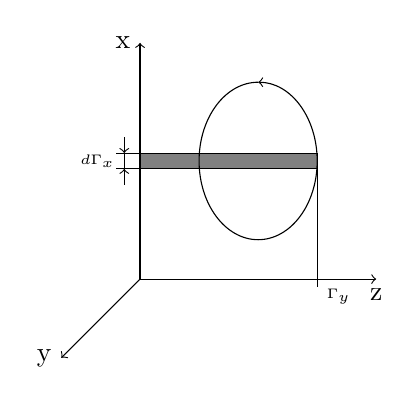
\begin{tikzpicture}
\label{img:rot_szx}
\draw[->] (0, 0) -- (3, 0);
\draw (3, 0) node[anchor=north]{z};

\draw[->] (0, 0) -- (0, 3);
\draw (0, 3) node[anchor=east]{x};

\draw[->] (0, 0) -- (-1, -1);
\draw (-1, -1) node[anchor=east]{y};

\filldraw[color=black, fill=gray] (0, 1.4) -- (2.25, 1.4) -- (2.25, 1.6) -- (0, 1.6) -- (0, 1.4);
\draw[->] (1.5, 2.5) arc (90:450:0.75 and 1);

\draw (0, 1.4) -- (-0.3, 1.4);
\draw (0, 1.6) -- (-0.3, 1.6);

\draw[->] (-0.2, 1.2) -- (-0.2, 1.4);
\draw (-0.2, 1.4) -- (-0.2, 1.6);
\draw (-0.2, 1.5) node[anchor=east]{\tiny \(d \Gamma_x\)};
\draw[->] (-0.2, 1.8) -- (-0.2, 1.6);

\draw (2.25, 1.4) -- (2.25, -0.1);
\draw (2.25, 0) node[anchor=north west]{\tiny \(\Gamma_y\)};
\end{tikzpicture}

Obdobně integrál \(\int_{t_1}^{t_2} \Gamma_y(t) \frac{d \Gamma_x}{dt} dt\) představuje plochu průmětu křivky \(\Gamma\) do roviny \(xy\), tentokrát však zápornou. Označíme ho proto \(-S_{xy}\).

\begin{equation}
\label{eq:rotace_3}
\begin{matrix}
-\frac{\partial v_x}{\partial y} S_{xy} + \frac{\partial v_x}{\partial z} S_{xz} \\
+ \frac{\partial v_y}{\partial x} S_{xy} - \frac{\partial v_y}{\partial z} S_{yz} \\
- \frac{\partial v_z}{\partial x} S_{xz} + \frac{\partial v_z}{\partial y} S_{yz}
\end{matrix}
\end{equation}

Úpravou pak získáme vztah \eqref{eq:rotace_4}.

\begin{equation}
\label{eq:rotace_4}
\left( \frac{\partial v_z}{\partial y} - \frac{\partial v_y}{\partial z} \right) S_{yz} + \left( \frac{\partial v_x}{\partial z} - \frac{\partial v_z}{\partial x} \right) S_{xz} + \left( \frac{\partial v_y}{\partial x} - \frac{\partial v_x}{\partial y} \right) S_{xy} 
\end{equation}

Dále budeme předpokládat, že smyčka leží v rovině (to jsme doposud nemuseli). Označme jednotkovou normálu této roviny \(n\). Pak \(S_{yz} = n_x S\), \(S_{xz} = n_y S\) a \(S_{xy} = n_z S\). Dosazením do vztahu \eqref{eq:rotace_4} získáme vztah \eqref{eq:rotace_5}.

\begin{equation}
\label{eq:rotace_5}
\left( \frac{\partial v_z}{\partial y} - \frac{\partial v_y}{\partial z} \right) n_x S + \left( \frac{\partial v_x}{\partial z} - \frac{\partial v_z}{\partial x} \right) n_y S + \left( \frac{\partial v_y}{\partial x} - \frac{\partial v_x}{\partial y} \right) n_z S 
\end{equation}

Vztah můžeme přepsat na skalární součin \eqref{eq:rotace_6}.

\begin{equation}
\label{eq:rotace_6}
S \cdot \vect{n} \cdot \left(\frac{\partial v_z}{\partial y} - \frac{\partial v_y}{\partial z}, \frac{\partial v_x}{\partial z} - \frac{\partial v_z}{\partial x}, \frac{\partial v_y}{\partial x} - \frac{\partial v_x}{\partial y} \right)
\end{equation}

Vektor na pravé straně skalárního součinu ve vztahu \eqref{eq:rotace_6} závisí pouze na poli \(v\), není závislý na smyčce \(\Gamma\). Nazveme ho rotací pole \(\vect{v}\) a označíme \(\rot \ \vect{v}\). Rotaci tedy lze spočítat posle vztahu \eqref{eq:rotace_vypocet}.

\begin{equation}
\label{eq:rotace_vypocet}
u = \rot \ \vect{v} = \left(\frac{\partial v_z}{\partial y} - \frac{\partial v_y}{\partial z}, \frac{\partial v_x}{\partial z} - \frac{\partial v_z}{\partial x}, \frac{\partial v_y}{\partial x} - \frac{\partial v_x}{\partial y} \right)
\end{equation}

Chceme-li rotaci zapsat ve složkovém tvaru, tak získáme 3 rovnice:

\begin{equation}
\begin{split}
u'_1 = \frac{\partial v'_3}{\partial P'_2} - \frac{\partial v'_2}{\partial P'_3} \\
u'_2 = \frac{\partial v'_1}{\partial P'_3} - \frac{\partial v'_3}{\partial P'_1} \\
u'_3 = \frac{\partial v'_2}{\partial P'_1} - \frac{\partial v'_1}{\partial P'_2}
\end{split}
\end{equation}

Pomocí Levi-Civitova tenzoru \(\varepsilon_{ijk}\) můžeme však všechny 3 rovnice zapsat pomocí jedné.

\begin{equation}
\label{eq:rotace_tenzorova}
\begin{split}
u'_i = \sum_{j=1}^3 \sum_{k=1}^3 \varepsilon_{ijk} \cdot \frac{\partial v'_k}{\partial P'_j}
\end{split}
\end{equation}

Vyjádřeme rotaci v křivočarých souřadnicích. Vztah \eqref{eq:rotace_tenzorova} vypadá, jako dvojí zůžení tenzoru, ale bohužel parciální derivace \(\frac{\partial v_k}{\partial P_j}\) nejsou tenzorem. Vztah tedy misíme upravit tak, aby veličiny v~něm obsažené tenzory byly:

\begin{equation}
\label{eq:rotace_tenzorova_2}
\begin{split}
u'_i = \frac{1}{2} \left(\sum_{j=1}^3 \sum_{k=1}^3 \varepsilon_{ijk} \cdot \frac{\partial v'_k}{\partial P'_j} + \sum_{j=1}^3 \sum_{k=1}^3 \varepsilon_{ijk} \cdot \frac{\partial v'_k}{\partial P'_j} \right) = \\
\frac{1}{2} \left(\sum_{j=1}^3 \sum_{k=1}^3 \varepsilon_{ijk} \cdot \frac{\partial v'_k}{\partial P'_j} + \sum_{k=1}^3 \sum_{j=1}^3 \varepsilon_{ikj} \cdot \frac{\partial v'_j}{\partial P'_k} \right) = \\
\frac{1}{2} \left(\sum_{j=1}^3 \sum_{k=1}^3 \varepsilon_{ijk} \cdot \frac{\partial v'_k}{\partial P'_j} + \sum_{j=1}^3 \sum_{k=1}^3 \varepsilon_{ikj} \cdot \frac{\partial v'_j}{\partial P'_k} \right) = \\
\frac{1}{2} \left(\sum_{j=1}^3 \sum_{k=1}^3 \varepsilon_{ijk} \cdot \frac{\partial v'_k}{\partial P'_j} - \sum_{j=1}^3 \sum_{k=1}^3 \varepsilon_{ijk} \cdot \frac{\partial v'_j}{\partial P'_k} \right) = \\
\frac{1}{2} \sum_{j=1}^3 \sum_{k=1}^3 \varepsilon_{ijk} \cdot \left(\frac{\partial v'_k}{\partial P'_j} - \frac{\partial v'_j}{\partial P'_k} \right)
\end{split}
\end{equation}

V~prvním kroku jsme vztah napsali polovinu dvojnásobku vztahu \eqref{eq:rotace_tenzorova}. Ve druhém kroku jsme provedli substituci \(j \leftrightarrow k\) u~druhého členu - prohodili jsme tyto proměnné. Ve třetím kroku jsme prohodily nezávislé sumy u~druhého členu. Ve čtvrtém kroku jsme prohodily indexy \(j\) a~\(k\), proto jsme museli otočit znaménko u~sumy. Nakonec jsme oba členy spojily. Podle vztahu~\eqref{eq:tenzor_rozdil_derivaci_vektoru} je rozdíl parciálních derivací, který jsme získaly, tenzorem druhého řádu. Rovnice \eqref{eq:rotace_tenzorova_2} je proto tenzorovou rovnicí a~můžeme ji tak proto transformovat:

\begin{equation}
\label{eq:rotace_tenzorova_3}
\begin{split}
u^i = \frac{1}{2} \sum_{j=1}^3 \sum_{k=1}^3 \epsilon^{ijk} \cdot \left(\frac{\partial v_k}{\partial P_j} - \frac{\partial v_j}{\partial P_k} \right) = \\
J' \cdot \frac{1}{2} \sum_{j=1}^3 \sum_{k=1}^3 \varepsilon_{ijk} \cdot \left(\frac{\partial v_k}{\partial P_j} - \frac{\partial v_j}{\partial P_k} \right) = \\
J' \cdot \sum_{j=1}^3 \sum_{k=1}^3 \varepsilon_{ijk} \cdot \frac{\partial v_k}{\partial P_j} = \\
= \sum_{j=1}^3 \sum_{k=1}^3 \epsilon^{ijk} \cdot \frac{\partial v_k}{\partial P_j}
\end{split}
\end{equation}

V~prvním kroku jsme zapsali transformovaný vztah \eqref{eq:rotace_tenzorova_2}, pak jsme rozepsali symbol \(\epsilon_{ijk} = J' \cdot \varepsilon_{ijk}\). Dále jsme využili obdobu vztahu \eqref{eq:rotace_tenzorova_2}, ale obráceně a~pro křivočaré souřadnice. Tento postup nebudu opět opakovat. Nakonec jsme opět přešli k~\(\epsilon\). Vidíme, že rotace transformuje tak, jak bychom čekali. Bez výše uvedeného odvození se však neobejdeme.


\subsection{Stokesova věta}

Mějme plochu \(S\) ohraničenou uzavřenou smyčkou \(\partial S\). Tuto plochu můžeme rozdělit na mnoho malých plošek \(\mathrm{d}S\), které můžeme považovat za rovinné útvary ohraničené uzavřenými křivkami \(\partial \mathrm{d}S\). V sekci \ref{sec:rotace} jsme odvodili vztah \eqref{eq:stokes_ds}.

\begin{equation}
\label{eq:stokes_ds}
\oint_{\partial \mathrm{d}S} \vect{v} \cdot d\vect{l} = (\rot \ \vect{v}) \cdot \vect{n} \cdot ds
\end{equation}

Máme-li 2 sousední plošky, pak se celková cirkulace po jejich vnější hranici sčítá podle vztahu \eqref{eq:deleni_cirkulace}. Jejich příspěvky \((\rot \ \vect{v}) \cdot \vect{n}\) se prostě sčítají. Proto si můžeme dovolit obě strany rovnice \eqref{eq:stokes_ds} integrovat a získáme tak rovnici \eqref{eq:stokesova_veta}. Ta se nazývá Stokesova věta a umožňuje nám přecházet mezi plošným integrálem po ploše \(S\) a křivkovým integrálem po její hranici \(\partial S\).

\begin{equation}
\label{eq:stokesova_veta}
\oint_{\partial S} \vect{v} \cdot d\vect{l} = \int_S (\rot \ \vect{v}) \cdot \vect{n} \cdot ds
\end{equation}


\section{Tok vektoru}

Pokud máme vektorové pole definované v~prostoru, tak můžeme určit jeho tok určenou plochou. Obdobně pokud máme vektorové pole definované
 v~rovině, tak můžeme určit jeho tok určenou křivkou. V~obou případech je tento tok roven integrálu průmětů vektorů pole do normál plochy nebo křivky násobené plochou nebo délkou elementu plochy nebo křivky.
 
Pokud vektorové pole představuje rychlost proudění tekutiny, pak tok vektoru představuje celkový průtok této tekutiny plochou nebo křivkou.

\subsection{Tok vektoru plochou v prostoru - plošný integrál}

Je-li \(S = \left(S_x(t, u), S_y(t, u), S_z(t, u)\right)\) po částech hladká plocha s jednotkovou normálou \(\vect{n}\) a \(\vect{v}\) je vektorové pole,
pak plošný integrál definujeme rovnicí \eqref{eq:plosny_integral_definice}. Říkáme mu tok vektoru \(v\) plochou \(S\).


\begin{equation}
\label{eq:plosny_integral_definice}
\begin{split}
\int_S \vect{v} \cdot d\vect{s} = \int_S \vect{v} \cdot \vect{n} ds
\end{split}
\end{equation}

Využijeme-li vztah \eqref{eq:element_plochy}, tak lze plošný integrál až na znaménko spočítat pomocí vztahu \eqref{eq:plosny_integral_vypocet}.

\begin{equation}
\label{eq:plosny_integral_vypocet}
\begin{split}
\int_S \vect{v} \cdot \vect{n} ds = \iint_S \vect{v} \cdot \left (\frac{\partial S}{\partial t} \times \frac{\partial S}{\partial u}\right) dt \ du
\end{split}
\end{equation}

Je-li plocha uzavřená, pak toto zdůrazníme kroužkem přes symbol integrálu, tedy \(\oint_S \vect{v} \cdot d\vect{s}\). Podle konvence pak normála \(n\) míří vně z plochy.

Například zákon kontinuity toku nestlačitelné kapaliny lze zapsat \(\oint_S \vect{v} \cdot d\vect{s} = 0\). Vyjadřuje fakt, že velkový výtok vektoru rychlosti kapaliny \(v\) jakoukoli uzavřenou plochou \(S\) je nulový, tedy že se kapalina nikde neztrácí, nevyvěrá ani nestlačuje. 

\subsection{Příklad}

Rychlost kapaliny je popsána vztahem \(v = \)

\subsection{Divergence}
\label{sec:divergence}

Vyšetřeme nyní tok vektoru nekonečně malou uzavřenou plochou. Vektorové pole \(\vect{v}\) linearizujeme podle vztahu \eqref{eq:divergence_linearizace}.
Předpokládáme, že pole pole je hladké - má derivace prvního řádu.

\begin{equation}
\label{eq:divergence_linearizace}
\vect{v} \approx \begin{pmatrix}
v_{x_0} + \frac{\partial v_x}{\partial x} \cdot x + \frac{\partial v_x}{\partial y} \cdot y + \frac{\partial v_x}{\partial z} \cdot z \\
v_{y_0} + \frac{\partial v_y}{\partial x} \cdot x + \frac{\partial v_y}{\partial y} \cdot y + \frac{\partial v_y}{\partial z} \cdot z \\
v_{z_0} + \frac{\partial v_z}{\partial x} \cdot x + \frac{\partial v_z}{\partial y} \cdot y + \frac{\partial v_z}{\partial z} \cdot z
\end{pmatrix}
\end{equation}

Dosadíme je do vztahu \eqref{eq:plosny_integral_definice} a získáme tak vztah \eqref{eq:divergence_1}

\begin{equation}
\label{eq:divergence_1}
\begin{split}
\int_S \vect{v} \cdot d\vect{s} = \oint_S \begin{pmatrix}
v_{x_0} + \frac{\partial v_x}{\partial x} \cdot x + \frac{\partial v_x}{\partial y} \cdot y + \frac{\partial v_x}{\partial z} \cdot z \\
v_{y_0} + \frac{\partial v_y}{\partial x} \cdot x + \frac{\partial v_y}{\partial y} \cdot y + \frac{\partial v_y}{\partial z} \cdot z \\
v_{z_0} + \frac{\partial v_z}{\partial x} \cdot x + \frac{\partial v_z}{\partial y} \cdot y + \frac{\partial v_z}{\partial z} \cdot z
\end{pmatrix} \cdot \vect{n} \mathrm{d}s
\end{split}
\end{equation}

Rozepsáním skalárního součinu a integrálu získáme výraz \eqref{eq:divergence_2}.

\begin{equation}
\label{eq:divergence_2}
\begin{matrix}
\int_S \vect{v} \cdot d\vect{s} = \\
v_{x_0} \oint_S n_x \mathrm{d}s + \frac{\partial v_x}{\partial x} \oint_S x n_x \mathrm{d}s + \frac{\partial v_x}{\partial y} \oint_S y n_x \mathrm{d}s + \frac{\partial v_x}{\partial z} \oint_S z n_x \mathrm{d}s + \\
v_{y_0} \oint_S n_y \mathrm{d}s + \frac{\partial v_y}{\partial x} \oint_S x n_y \mathrm{d}s + \frac{\partial v_y}{\partial y} \oint_S y n_y \mathrm{d}s + \frac{\partial v_y}{\partial z} \oint_S z n_y \mathrm{d}s + \\
v_{z_0} \oint_S n_z \mathrm{d}s + \frac{\partial v_z}{\partial x} \oint_S x n_z \mathrm{d}s + \frac{\partial v_z}{\partial y} \oint_S y n_z \mathrm{d}s + \frac{\partial v_z}{\partial z} \oint_S z n_z \mathrm{d}s
\end{matrix}
\end{equation}

Rozeberme první řádek součtu ve výrazu \eqref{eq:divergence_2}. Vyskytují se zde 4 integrály a ve všech se vyskytuje člen \(n_x \mathrm{d}s\). Ten představuje obsah průmětu plochy \(\mathrm{d}s\) do roviny kolmé k ose x, tedy do roviny y-z.

Jednak je zde integrál \(\oint_S x n_x \mathrm{d}s\). Uvědomíme-li si, že \(x n_x \mathrm{d}s\) je objem obecného válce se základnou tvořenou průmětem plochy \(\mathrm{d}s\) do roviny y-z a~výškou \(x\), pak \(\oint_S x n_x \mathrm{d}s = V\) je objem tělesa ohraničeného plochou \(S\).

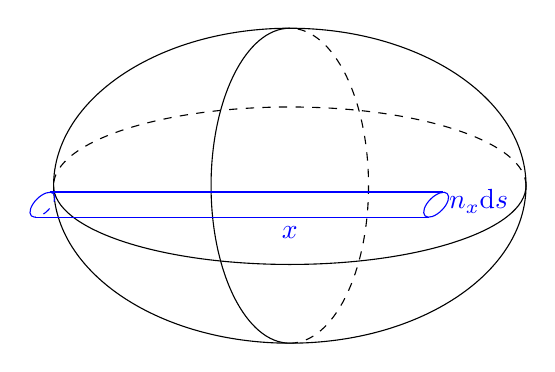
\begin{tikzpicture}
\label{img:objem}

\drawaxes{0}{0}{6}{4}{2}

\draw[thin] (5, 1) arc (0:360:3 and 2);

\draw[dashed] (5, 1) arc (0:180:3 and 1);
\draw[thin] (-1, 1) arc (180:360:3 and 1);

\draw[thin] (2, 3) arc (90:270:1 and 2);
\draw[dashed] (2, -1) arc (270:450:1 and 2);

\draw[color=blue, thin, rotate around={-45:(-1, 0.9)}] (-1, 0.9) arc (90:270:0.1 and 0.2);
\draw[color=blue, dashed, rotate around={-45:(-1, 0.9)}] (-1, 0.9) arc (90:-90:0.1 and 0.2);

\draw[color=blue, thin, rotate around={-45:(4, 0.9)}] (4, 0.9) arc (90:450:0.1 and 0.2);

\draw[color=blue, thin] (-1.05, 0.92) -- (3.95, 0.92);
\draw[color=blue, thin] (-1.23, 0.6) -- (3.77, 0.6);

\draw[color=blue] (3.9, 0.8) node[anchor=west]{\(n_x \mathrm{d}s\)};
\draw[color=blue] (2.0, 0.6) node[anchor=north]{\(x\)};

\end{tikzpicture}

Další 3 integrály jsou typu \(\oint_S f(y, z) n_x \mathrm{d}s\). Uvažujme průmět plochy \(S\) do roviny y-z. Protože je plocha \(S\) uzavřená, tak každým bodem \([y, z]\) projde sudý počet krát, přičemž v polovině případů bude normála plochy orientována v kladném směru osy x, kdy součin \(n_x \mathrm{d}s\) bude kladný, a v polovině případů bude normála plochy orientována v záporném směru osy x, kdy součin \(n_x \mathrm{d}s\) bude záporný. Protože funkce \(f(y, z)\) závisí pouze na souřadnicích \(y\) a \(z\), proto je její funkční hodnota v obou případech stejná a v integrálu se vyruší. Proto \(\oint_S f(y, z) n_x \mathrm{d}s = 0\). Zopakujeme-li uvedený postup pro všechny řádky, získáme vztah \eqref{eq:divergence_3}.

\begin{equation}
\label{eq:divergence_3}
\int_S \vect{v} \cdot d\vect{s} = \frac{\partial v_x}{\partial x} V + \frac{\partial v_y}{\partial y} V + \frac{\partial v_z}{\partial z} V = \left(\frac{\partial v_x}{\partial x} + \frac{\partial v_y}{\partial y} + \frac{\partial v_z}{\partial z}\right) V
\end{equation}
\
Ve výrazu \eqref{eq:divergence_3} se vyskytuje součet, který je závislý pouze na poli \(v\) a nazveme jej divergence pole \(v\). 

\begin{equation}
\label{eq:divergence_definice}
\diverg \vect{v} = \frac{\partial v_x}{\partial x} + \frac{\partial v_y}{\partial y} + \frac{\partial v_z}{\partial z}
\end{equation}

Divergence je definována vztahem \eqref{eq:divergence_definice} a představuje tedy výtok pole \(v\) z nekonečně malého tělesa dělená jeho objemem.

Vyjádřeme divergenci v~křivočarých souřadnicích. Začněme zápisem divergence ve složkovém tvaru:

\begin{equation}
\diverg \vect{v} = \sum_{i=1}^n \frac{\partial v_i}{\partial P'_i}
\end{equation}

Dosadíme-li za derivace vztah \eqref{eq:derivace_vektoru}, získáme:

\begin{equation}
\begin{split}
\diverg \vect{v} = \sum_{i=1}^n \sum_{k=1}^n \sum_{l=1}^n \frac{\partial p_k}{\partial P'_i} \frac{\partial p_l}{\partial P'_i} \frac{\partial v_k}{\partial P_l} + \sum_{i=1}^n \sum_{k=1}^n \frac{\partial^2 p_k}{\partial P'^2_i} v_k = \\
\sum_{k=1}^n \sum_{l=1}^n g^{kl} \frac{\partial v_k}{\partial P_l} + \sum_{i=1}^n \sum_{k=1}^n \frac{\partial^2 p_k}{\partial P'^2_i} v_k = \\
\sum_{k=1}^n \sum_{l=1}^n g^{kl} \frac{\partial v_k}{\partial P_l} + \sum_{k=1}^n v_k \cdot \sum_{i=1}^n \frac{\partial^2 p_k}{\partial P'^2_i}
\end{split}
\end{equation}

\subsection{Vlastnosti toku pole}

Vyšetřeme nyní, jak se chová tok pole při dělení plochy na menší. Mějme uzavřenou plochu \(S_S\), kterou rozdělíme libovolnou přepážkou \(S_P\) na 2 uzavřené plochy \(S_1\) a \(S_2\). Přepážka je tvořena dvěma opačně orientovanými částmi plochy, které jsou nekonečně blízké. Proto se jejich příspěvky do celkového toku vyruší a platí tak vztah \eqref{eq:deleni_toku}.

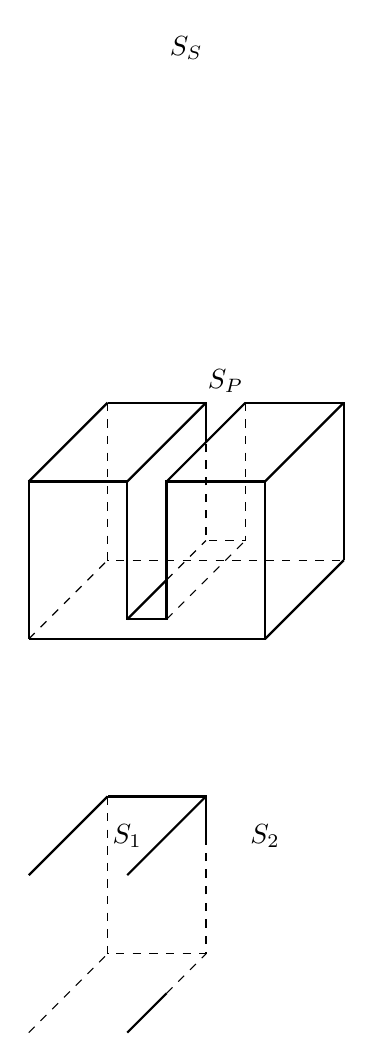
\begin{tikzpicture}
\label{img:deleni_toku}

--== One box ==--

\pgfmathsetmacro{\x}{0}
\pgfmathsetmacro{\y}{10}
\pgfmathsetmacro{\d}{1.0}

\drawaxes{\x}{\y}{4.5}{3}{2}
\drawbox{\x - 0.5}{\y - 1.5}{\x + 2.5}{\y + 0.5}{\d};

\draw (\x + 1.5, \y + 1.0) node[anchor=center]{\(S_S\)};


--== Splitted box ==--

\pgfmathsetmacro{\x}{0}
\pgfmathsetmacro{\y}{5}

\drawaxes{\x}{\y}{4.5}{3}{2}

-- Front
\draw[thick] (\x - 0.5, \y - 1.5) -- (\x + 2.5, \y - 1.5) -- (\x + 2.5, \y + 0.5) -- (\x + 1.25, \y + 0.5) -- (\x + 1.25, \y - 1.25) -- (\x + 0.75, \y - 1.25) -- (\x + 0.75, \y + 0.5) -- (\x - 0.5, \y + 0.5) -- (\x - 0.5, \y - 1.5);

\draw[dashed] (\x - 0.5 + \d, \y + 0.5 + \d) -- (\x - 0.5 + \d, \y - 1.5 + \d) -- (\x + 2.5 + \d, \y - 1.5 + \d);
\draw[thick] (\x + 2.5 + \d, \y - 1.5 + \d) -- (\x + 2.5 + \d, \y + 0.5 + \d) -- (\x + 1.25 + \d, \y + 0.5 + \d);
\draw[dashed] (\x + 1.25 + \d, \y + 0.5 + \d) -- (\x + 1.25 + \d, \y - 1.25 + \d) -- (\x + 0.75 + \d, \y - 1.25 + \d) -- (\x + 0.75 + \d, \y + 0.0 + \d);
\draw[thick] (\x + 0.75 + \d, \y + 0.0 + \d) -- (\x + 0.75 + \d, \y + 0.5 + \d) -- (\x - 0.5 + \d, \y + 0.5 + \d);

\draw[dashed] (\x - 0.5, \y - 1.5) -- (\x - 0.5 + \d, \y - 1.5 + \d);
\draw[thick] (\x + 2.5, \y - 1.5) -- (\x + 2.5 + \d, \y - 1.5 + \d);
\draw[thick] (\x + 2.5, \y + 0.5) -- (\x + 2.5 + \d, \y + 0.5 + \d);
\draw[thick] (\x + 1.25, \y + 0.5) -- (\x + 1.25 + \d, \y + 0.5 + \d);
\draw[dashed] (\x + 1.25, \y - 1.25) -- (\x + 1.25 + \d, \y - 1.25 + \d);
\draw[thick] (\x + 0.75, \y - 1.25) -- (\x + 0.75 + \d / 2, \y - 1.25 + \d / 2);
\draw[dashed] (\x + 0.75 + \d / 2, \y - 1.25 + \d / 2) -- (\x + 0.75 + \d, \y - 1.25 + \d);
\draw[thick] (\x + 0.75, \y + 0.5) -- (\x + 0.75 + \d, \y + 0.5 + \d);
\draw[thick] (\x - 0.5, \y + 0.5) -- (\x - 0.5 + \d, \y + 0.5 + \d);

\draw (\x + 2.0, \y + 1.5) node[anchor=south]{\(S_P\)};


--== Two boxes ==--

\pgfmathsetmacro{\x}{0}
\pgfmathsetmacro{\y}{0}

\drawaxes{\x}{\y}{4.5}{3}{2}

-- Front rectangle
\pgfmathsetmacro{\ax}{\x - 0.5}
\pgfmathsetmacro{\ay}{\y - 1.5}
\pgfmathsetmacro{\bx}{\x + 0.75}
\pgfmathsetmacro{\by}{\y + 0.5}
\drawrect{\ax}{\ay}{\bx}{\by}{thick};

-- Rear rectangle
\draw[dashed] (\ax + \d, \by + \d) -- (\ax + \d, \ay + \d) -- (\bx + \d, \ay + \d) -- (\bx + \d, \y + 1.0);
\draw[thick] (\bx + \d, \y + 1.0) -- (\bx + \d, \by + \d) -- (\ax + \d, \by + \d);

-- Z edges
\draw[dashed] (\ax, \ay) -- (\ax + \d, \ay + \d);
\draw[thick] (\bx, \ay) -- (\bx + \d / 2, \ay + \d / 2);
\draw[dashed] (\bx + \d / 2, \ay + \d / 2) -- (\bx + \d, \ay + \d);
\draw[thick] (\bx, \by) -- (\bx + \d, \by + \d);
\draw[thick] (\ax, \by) -- (\ax + \d, \by + \d);

\drawbox{\x + 1.25}{\y - 1.5}{\x + 2.5}{\y + 0.5}{1.0};

\draw (\x + 0.75, \y + 1.0) node[anchor=center]{\(S_1\)};
\draw (\x + 2.5, \y + 1.0) node[anchor=center]{\(S_2\)};

\end{tikzpicture}


\begin{equation}
\label{eq:deleni_toku}
\oint_{S_S} \vect{v} \cdot \mathrm{d}\vect{s} = \oint_{S_1} \vect{v} \cdot \mathrm{d}\vect{s} + \oint_{S_2} \vect{v} \cdot \mathrm{d}\vect{s}
\end{equation}


\subsection{Gaussův teorém}

Ze vztahu \eqref{eq:divergence_3} můžeme odvodit vztah \eqref{eq:gauss_dv} pro výpočet toku pole elementární uzavřenou ploškou \(\partial \mathrm{d}V\).

\begin{equation}
\label{eq:gauss_dv}
\int_{\partial \mathrm{d}V} \vect{v} \cdot d\vect{s} = \left(\diverg \ \vect{v} \right) \mathrm{d}V
\end{equation}


Podle vztahu \label{eq:deleni_toku} víme, že se toky sousedními ploškami sčítají, přičemž společné části ploch se vyruší. Proto pokud budeme integrovat
vztah \eqref{eq:gauss_dv} přes těleso \(V\), tak plošný integrál přejde na plochu po povrchu tělesa \(V\). Získáme tak Gaussův teorém \eqref{eq:gauss}.

\begin{equation}
\label{eq:gauss}
\oint_{\partial V} \vect{v} \cdot d\vect{s} = \int_V \left(\diverg \ \vect{v} \right) \mathrm{d}V
\end{equation}




\subsection{Tok vektoru křivkou v~rovině}

Je-li \(l = \left(l_x(t), l_y(t)\right)\) po částech hladká plocha s jednotkovou normálou \(\vect{n}\) a \(\vect{v}\) je vektorové pole,
pak tok vektoru \(v\) křivkou \(l\) definujeme rovnicí \eqref{eq:tok_krivkou_definice}.

\begin{equation}
\label{eq:tok_krivkou_definice}
\begin{split}
\int_l \vect{v} \cdot \vect{n} dl
\end{split}
\end{equation}

Máme-li vektor \(d \vect{l} = \left(\frac{d l_x}{dt}, \frac{d l_y}{dt}\right)\), pak vektor k~němu kolmý získáme tak, že prohodíme souřadnice a~u~jedné z~nich otočíme znaménko. Proto \(\vect{n} dl = \left(\frac{d l_y}{dt}, -\frac{d l_x}{dt}\right) dt\). Tok vektoru \(v\) křivkou \(l\) proto můžeme až na znaménko vypočítat podle vztahu \eqref{eq:tok_krivkou_vypocet}.

\begin{equation}
\label{eq:tok_krivkou_vypocet}
\begin{split}
\int_{t_1}^{t_2} \left (v_x \cdot \frac{d l_y}{dt} -v_y \cdot \frac{d l_x}{dt} \right) dt
\end{split}
\end{equation}

\subsection{Greenův teorém}

Obdobou Gaussova teorému v prostoru je Greenův teorém v rovině. Je možné jej odvodit obdobně jako Gaussův teorém.

My jej odvodíme z Gaussova teorému následující úvahou. Nechť je pole \(v\) konstantní ve směru osy \(z\). Těleso \(V\) zvolíme ve formě obecného válce, tedy libovolné podstavy protažené ve směru osy \(z\). Jeho podstavu označme \(S_P\), její hranici \(\partial S_P\) a v výšku válce \(h\).

Vyjděme z Gaussova teorému v rovnici \eqref{eq:green_1}.

\begin{equation}
\label{eq:green_1}
\oint_{\partial V} \vect{v} \cdot d\vect{s} = \int_V \left(\diverg \ \vect{v} \right) \mathrm{d}V
\end{equation}

Tok pole plochou na levé straně rovnice můžeme rozepsat na součet toku pole podstavami a pláštěm válce.
To pláštěm válce je tok hranicí podstavy násobené výškou válce, protože je pole po celé výšce konstantní. Tok podstavami je nulový, protože je pole konstantní ve směru osy \(z\) a tudíž jeho průmět do normály postavy je nulový.

Stejně tak můžeme nahradit objemový integrál na pravé straně rovnice plošným integrálem násobeným výškou. Získáme tak rovnici \eqref{eq:green_2}.

\begin{equation}
\label{eq:green_2}
h \oint_{\partial S_P} \vect{v} \cdot d\vect{l} = h \int_{S_P} \left(\diverg \ \vect{v} \right) \mathrm{d}S
\end{equation}

Podělíme-li rovnici \eqref{eq:green_2} výškou \(h\) a přejmenujeme plochu, tak získáme rovnici \eqref{eq:greenuv_teorem}. Uvědomme si, že \(\frac{\partial v_z}{\partial z} = 0\).
Proto divergence v prostoru, se kterou jsme dosud pracovali, je shodná s divergencí v rovině.

\begin{equation}
\label{eq:greenuv_teorem}
\oint_{\partial S} \vect{v} \cdot d\vect{l} = h \int_S \left(\diverg \ \vect{v} \right) \mathrm{d}S
\end{equation}

Uvedený postup je obecně použitelný, pokud máme problém definovaný v prostoru, ale v jedné nebo více os je invariantní vůči posunutí. Můžeme tak snížit
počet dimenzi problému.
